\documentclass[conference]{IEEEtran}
\IEEEoverridecommandlockouts

\usepackage{float}
\usepackage{cite}
\usepackage{amsmath,amssymb,amsfonts}
\usepackage{algorithmic}
\usepackage{graphicx}
\usepackage{textcomp}
\usepackage{xcolor}
\usepackage{listings}
\usepackage{booktabs}
\usepackage{array} 
\usepackage{url}

% Mendefinisikan warna kustom untuk syntax highlighting
\definecolor{codeBackground}{rgb}{0.96,0.96,0.96} % Abu-abu sangat terang
\definecolor{codeComment}{rgb}{0.0, 0.5, 0.0}     % Hijau
\definecolor{codeKeyword}{rgb}{0.0, 0.0, 0.8}     % Biru tua
\definecolor{codeString}{rgb}{0.6, 0.1, 0.1}      % Merah marun
\definecolor{codeNumber}{rgb}{0.5, 0.5, 0.5}      % Abu-abu

% Membuat style khusus bernama "PictureStyle"
\lstdefinestyle{PictureStyle}{
    language=C,
    backgroundcolor=\color{codeBackground},   
    commentstyle=\color{codeComment}\itshape,
    keywordstyle=\color{codeKeyword}\bfseries,
    numberstyle=\tiny\color{codeNumber},
    stringstyle=\color{codeString},
    basicstyle=\ttfamily\footnotesize, % Menggunakan font mesin tik ukuran kecil
    breakatwhitespace=false,         
    breaklines=true,                 % Auto-wrap text jika terlalu panjang
    captionpos=b,                    % Posisi caption di bawah (bottom)
    keepspaces=true,                 
    numbers=left,                    % Nomor baris di sebelah kiri
    numbersep=8pt,                  
    showspaces=false,                
    showstringspaces=false,
    showtabs=false,                  
    tabsize=2,
    frame=single,                    % Bingkai kotak penuh di sekeliling kode
    rulecolor=\color{black!30},      % Warna bingkai abu-abu gelap
    xleftmargin=15pt,                % Margin kiri agar nomor baris tidak menabrak batas
    framexleftmargin=15pt
}

\def\BibTeX{{\rm B\kern-.05em{\sc i\kern-.025em b}\kern-.08em
    T\kern-.1667em\lower.7ex\hbox{E}\kern-.125emX}}
\begin{document}

\title{Design of Custom Instructions on PicoRV32 Processor for Accelerating Fast Fourier Transform Algorithm}

\author{\IEEEauthorblockN{1\textsuperscript{st} Abidul Qohar}
\IEEEauthorblockA{\textit{Department of Electrical Engineering} \\
\textit{and Information Technology} \\
\textit{Faculty of Engineering}\\
\textit{Universitas Gadjah Mada} \\
Yogyakarta, Indonesia \\
abidulqohar@mail.ugm.ac.id}
\and
\IEEEauthorblockN{2\textsuperscript{nd} Agus Bejo}
\IEEEauthorblockA{\textit{Department of Electrical Engineering} \\
\textit{and Information Technology} \\
\textit{Faculty of Engineering}\\
\textit{Universitas Gadjah Mada} \\
Yogyakarta, Indonesia \\
agusbj@ugm.ac.id}
\and
\IEEEauthorblockN{3\textsuperscript{rd} Eka Firmansyah}
\IEEEauthorblockA{\textit{Department of Electrical Engineering} \\
\textit{and Information Technology} \\
\textit{Faculty of Engineering}\\
\textit{Universitas Gadjah Mada} \\
Yogyakarta, Indonesia \\
eka.firmansyah@ugm.ac.id}
}

\maketitle

\begin{abstract}
Audio equalizer applications rely on the Fast Fourier Transform (FFT) to
transform time-domain signals into the frequency domain for selective gain
adjustment. On resource-constrained embedded processors implementing only the
base RV32I integer instruction set, FFT computation becomes a performance
bottleneck due to the absence of hardware multiplication support and the
repetitive nature of the butterfly operation. This paper presents the
implementation of custom RISC-V instructions to accelerate the butterfly
computation of a radix-2 FFT integrated into a PicoRV32-based audio equalizer
system. Four custom instructions---mshift, bload, bfly, and bget are designed to
collapse the four input, two output butterfly operation into a single
hardware-accelerated sequence and minimize the multiplication operations through
the PicoRV32 Custom Peripheral Interface (PCPI). The GNU assembler is modified
to recognize the new instructions, enabling their use through inline assembly in
C code without requiring compiler backend changes. A complete System-on-Chip is
implemented in Verilog comprising the PicoRV32 core, the FFT custom instruction
module, ROM and dual RAM blocks, and AXI bus interconnect. Experimental results
from Icarus Verilog simulation show that processing 1024 audio samples through a
64-point FFT, 3-band equalizer, and inverse FFT requires 5.84 million
clock cycles with custom instructions enabled, compared to around 17.08 million
cycles in the software-only baseline a speedup of 2.92×. Functional
correctness is verified against a NumPy double-precision floating-point
reference, achieving a signal-to-noise ratio of 56.28 dB. These results
demonstrate that profile-driven custom instruction design is an effective
strategy for accelerating signal processing workloads on minimal RISC-V cores.
\end{abstract}

\begin{IEEEkeywords}
RISC-V, custom instruction, Fast Fourier Transform, audio equalizer, PicoRV32, hardware acceleration
\end{IEEEkeywords}

\section{Introduction}
Audio signal processing on embedded systems has become increasingly important
for applications such as smart speakers, hearing aids, in-vehicle audio systems,
and wearable devices \cite{stefani2022}. A common operation in these systems is
the audio equalizer, which selectively amplifies or attenuates specific
frequency bands of an audio signal. Modern equalizer implementations typically
transform the signal into the frequency domain using the Fast Fourier Transform
(FFT), apply per-band gain coefficients, and reconstruct the time-domain output
via the inverse FFT. The FFT, while asymptotically efficient at $O(N \log N)$,
imposes significant computational cost on embedded processors. The algorithm
consists of two principal stages: bit reversal permutation of the input indices,
and $\log_2(N)$ stages of butterfly operations, each involving complex-number
multiplication and addition \cite{cooley1965}. When executed on a
general-purpose processor implementing only the base RV32I instruction set,
which lacks hardware integer multiplication, each butterfly multiplication must
be emulated through sequences of shift and add instructions, dramatically
inflating the cycle count. RISC-V, an open and royalty-free instruction set
architecture, addresses this limitation through its modular design philosophy.
The specification reserves opcode space for user-defined custom instructions,
allowing designers to extend the base ISA with application-specific operations
without modifying the standard \cite{waterman2019}. This extensibility makes
RISC-V particularly suitable for domain-specific acceleration of computational
bottlenecks. Prior work has explored instruction set extensions to accelerate
FFT and related digital signal processing workloads. One line of research
integrates dedicated FFT coprocessors with RISC-V cores through specialized
coupling interfaces, in which a large block of the transform is offloaded to
custom hardware \cite{cao2025}, \cite{hu2021}. Such designs deliver substantial
acceleration but rely on heavyweight coprocessor interfaces and incur
significant area overhead, which is difficult to justify on minimal embedded
cores. A second line of work targets DSP workloads more broadly, extending the
RISC-V ISA for audio denoising \cite{yuan2022} and ultra-low-power wireless
signal processing \cite{belhadj2022}, while custom instructions for FFT on
non-RISC-V soft cores have also been investigated \cite{sundararajana2016}.
These approaches, however, are generally evaluated on processors that already
provide hardware integer multiplication through the standard M extension, so the
cost of emulating multiplication in software is not part of the problem they
address.

Few studies have considered the combined effect of two constraints that
characterize minimal RISC-V cores such as PicoRV32: the absence of the M
extension, which forces every multiplication to be emulated in software, and the
limited two-source operand bandwidth of a lightweight custom-instruction
interface, which is insufficient for the four-operand butterfly. The specific
access pattern of FFT-based audio equalization on such a core, where both of
these constraints act simultaneously, has not been directly addressed. This
paper targets that gap. It presents a profile-driven custom instruction design
that resolves both constraints on an unmodified PicoRV32 core, using only the
standard PicoRV32 Custom Peripheral Interface (PCPI) and without introducing a
separate coprocessor or modifying the core pipeline.

\section{Background}

\subsection{Fast Fourier Transform and the Butterfly Operation}

The Discrete Fourier Transform (DFT) of an $N$-point complex sequence $x[n]$ is
defined as~\cite{oppenheim} equation 1.
\begin{equation}
X[k] = \sum_{n=0}^{N-1} x[n] \cdot W_N^{nk}, \quad W_N = e^{-j2\pi/N}
\end{equation}

Direct computation requires $O(N^2)$ complex multiplications. The radix-2
decimation-in-time FFT reduces this to $O(N \log_2 N)$ by recursively
decomposing the DFT into smaller transforms, exploiting the periodicity and
symmetry of the twiddle factor $W_N$ \cite{cooley1965,oppenheim}. The algorithm
comprises two stages. The first stage is bit reversal, reorders the input
sequence by reversing the binary representation of each index. For $N = 8$, for
example, index 1 (binary 001) is swapped with index 4 (binary 100), and index 3
(011) is swapped with index 6 (110).

\begin{figure}[h!]
\centering
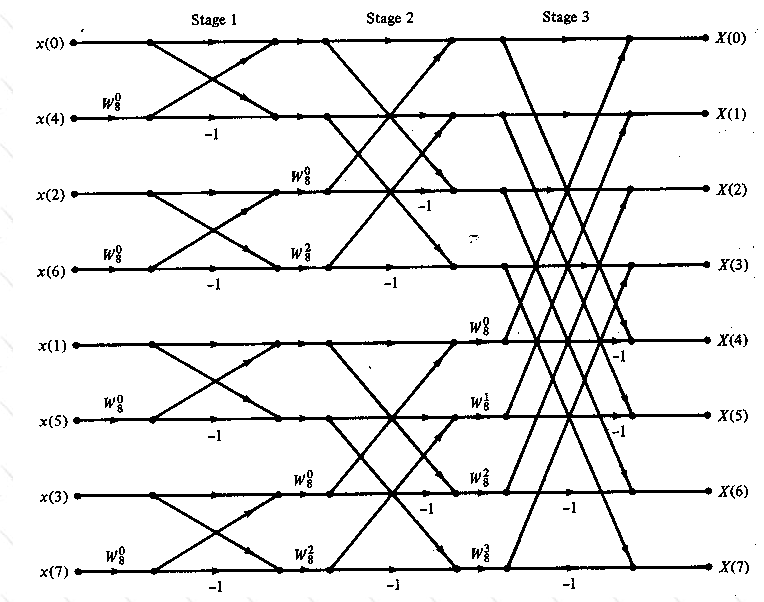
\includegraphics[width=0.81\columnwidth]{fft butterfly.png}
\caption{Butterfly unit process with 8 input data points to obtain frequency domain output \cite{cmlabfft}}
\label{fig:bfly}
\end{figure}

The second stage shown in Fig.~\ref{fig:bfly} performs $\log_2(N)$ passes of
butterfly operations. Each butterfly combines two complex inputs $a$ and $b$
using a twiddle factor $W_N^r$ to produce two outputs, requiring four real
multiplications and two real additions~\cite{oppenheim} :
\begin{equation}
A = a + W_N^r \cdot b
\end{equation}
\begin{equation}
B = a - W_N^r \cdot b
\end{equation}

Expanding the complex multiplication $W_N^r \cdot b$ where $W_N^r = c - js$ ($c
= \cos$, $s = \sin$) and $b = b_r + jb_i$:
\begin{equation}
\text{tr} = c \cdot b_r + s \cdot b_i
\end{equation}
\begin{equation}
\text{ti} = c \cdot b_i - s \cdot b_r
\end{equation}

A single butterfly therefore requires four real multiplications and two real
additions/subtractions. For an $N$-point FFT, the total number of butterfly
operations is $(N/2) \cdot \log_2(N)$. For $N = 64$, this yields 192
butterflies, each requiring four multiplications totaling 768 multiplications
per FFT.

\subsection{PicoRV32 Architecture}
PicoRV32 is a size-optimized RISC-V soft-core processor that implements the base
RV32I integer instruction set, with the RV32IM and RV32IMC extensions available
as optional configuration parameters~\cite{picorv32}. The core uses a sequential,
non-pipelined execution model in which each instruction completes before the
next is fetched; this simplicity both reduces area and simplifies the
integration of custom hardware, since there is no pipeline hazard logic to
disturb.

Two architectural properties of the configuration used in this work directly
shape the design problem addressed by this paper. First, the core is configured
as a pure RV32I implementation, without the \texttt{M} extension, so it provides
no hardware integer multiplier. Every multiplication in compiled code is
therefore expanded by the compiler into a sequence of shift and add
instructions, an emulation cost that is incurred on every multiply and is
quantified in Section~III.

Second, the core does not implement a hardware Floating-Point Unit (FPU) and
does not provide the RISC-V standard \texttt{F} extension, again to preserve a
minimal area footprint. As a consequence, any use of IEEE-754 floating-point
arithmetic would force the compiler to rely on software emulation (soft-float),
in which each floating-point operation expands into a long sequence of integer
instructions. For the latency-critical inner loops of a real-time audio
equalizer, this overhead is prohibitive. The absence of an FPU is therefore the
architectural reason that this work adopts a fixed-point numerical format,
described in Section~II-D.

\subsection{The PCPI Interface}

To allow the instruction set to be extended without modifying the core itself,
PicoRV32 provides the PicoRV32 Custom Peripheral Interface (PCPI) as in
Listing~\ref{lst:pcpi}.

% \begin{figure}[h!]
% \centering
% 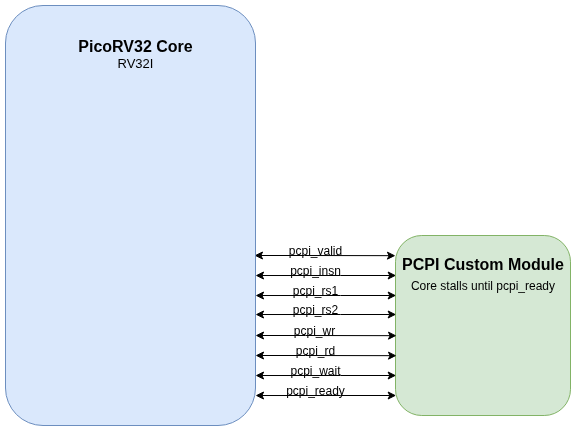
\includegraphics[width=0.81\columnwidth]{pcpi_flow.png}
% \caption{Pico Co-Processor Interface (PCPI) interaction flow}
% \label{fig:pcpi}
% \end{figure}

\begin{lstlisting}[style=PictureStyle, caption={PCPI Signals Interface in PicoRV32}, label={lst:pcpi}]
	// Pico Co-Processor Interface (PCPI)
	output reg        pcpi_valid,
	output reg [31:0] pcpi_insn,
	output     [31:0] pcpi_rs1,
	output     [31:0] pcpi_rs2,
	input             pcpi_wr,
	input      [31:0] pcpi_rd,
	input             pcpi_wait,
	input             pcpi_ready,
\end{lstlisting}

When the core fetches an instruction whose opcode is not part of the implemented
base ISA, it does not raise an illegal-instruction trap. Instead, it forwards
the complete 32-bit instruction word together with the two source register
values (\texttt{rs1} and \texttt{rs2}) onto the PCPI bus. An attached PCPI
module inspects the instruction, decodes its \texttt{funct3} and \texttt{funct7}
fields to select the requested operation, performs the computation, and signals
completion by asserting \texttt{pcpi\_ready}. A result value may optionally be
returned to the core through the \texttt{pcpi\_rd} signal, which the core writes
back to the destination register. During this exchange the core enters a stall
state and waits until \texttt{pcpi\_ready} is asserted, so the custom operation
may take a single cycle or multiple cycles without any change to the core's
control logic.

Because this mechanism leaves the PicoRV32 pipeline, register file, and decoder
untouched, a custom instruction module can be attached purely as an external
block. It allows the proposed FFT instructions to be added and verified without
forking or re-validating the core itself.

\subsection{Fixed-Point Arithmetic}

Because the PicoRV32 core used in this work provides no hardware FPU
(Section~II-B), all FFT computations are carried out in fixed-point arithmetic,
which maps directly onto the available RV32I integer datapath. In a fixed-point
representation, a real number is stored in an ordinary integer register, and the
binary point is fixed at a position agreed upon by convention rather than
encoded in the data. A $\mathrm{Q}m.f$ format denotes a signed value with $m$
integer bits and $f$ fractional bits, so the stored integer corresponds to the
real value scaled by $2^{f}$. Arithmetic on these values then reduces to
ordinary integer arithmetic on the scaled representation, which is exactly what
the RV32I instruction set provides. Sample data uses a Q21.10 representation: a
signed 32-bit integer with 1 sign bit, 21 integer bits, and 10 fractional bits.

% In this work, sample data uses a Q21.10 representation: a signed 32-bit integer
% with 1 sign bit, 21 integer bits, and 10 fractional bits. This gives a
% resolution of $2^{-10} \approx 1/1024$ and a representable range of
% approximately $\pm 2{,}097{,}152$, which is sufficient to hold both the input
% audio samples and the intermediate values that grow in magnitude through
% successive FFT stages. Twiddle factors are bounded to $[-1, +1]$ and therefore
% require no large integer range; they use a more compact Q5.10 representation in
% 16 bits, which still provides 10 fractional bits of precision for the $\sin$ and
% $\cos$ values.

\section{Custom Instruction Design}

\subsection{Profiling and Bottleneck Identification}

To establish a baseline for acceleration, the audio equalizer application was
first executed on a standard RV32I architecture without custom extensions. An
instruction-level profiling trace \cite{riscvprofiler} was generated to analyze
the execution behavior of the Fast Fourier Transform (FFT) during the real-time
audio buffering loop.

Table~\ref{tab:profiling} presents the ten most frequent instruction pairs
observed in the compiled FFT routine. The profiling reveals that
shift-and-add patterns dominate the instruction stream, with
\texttt{srli}--\texttt{slli}, \texttt{andi}--\texttt{beqz}, and
\texttt{slli}--\texttt{andi} together accounting for over 840{,}000 dynamic
instructions. These patterns arise from two sources: bit reversal index
manipulation (the \texttt{andi}--\texttt{beqz} and shift sequences for index bit
operations) and software emulation of multiplication in the butterfly
computation (the \texttt{slli}--\texttt{add} chains, which implement
shift-and-add multiplication in the absence of a hardware multiplier).
\begin{table}[h!]
\caption{Top 10 looping Instruction Pairs in the Compiled Audio Equalizer (RV32I)}
\label{tab:profiling}
\centering
\begin{tabular}{@{}clr@{}}
\toprule
\textbf{Rank} & \textbf{Instruction Pair} & \textbf{Count} \\
\midrule
1 & \texttt{srli} $\rightarrow$ \texttt{slli} & 291{,}707 \\
2 & \texttt{andi} $\rightarrow$ \texttt{beqz} & 289{,}144 \\
3 & \texttt{slli} $\rightarrow$ \texttt{andi} & 260{,}037 \\
4 & \texttt{lw} $\rightarrow$ \texttt{slli} & 94{,}403 \\
5 & \texttt{add} $\rightarrow$ \texttt{lw} & 62{,}111 \\
6 & \texttt{lw} $\rightarrow$ \texttt{sub} & 29{,}228 \\
7 & \texttt{addi} $\rightarrow$ \texttt{ble} & 29{,}124 \\
8 & \texttt{slli} $\rightarrow$ \texttt{mv} & 28{,}641 \\
9 & \texttt{mv} $\rightarrow$ \texttt{andi} & 28{,}532 \\
10 & \texttt{sub} $\rightarrow$ \texttt{sw} & 26{,}913 \\
\bottomrule
\end{tabular}
\end{table}

This instruction distribution exposes a severe bottleneck. The fundamental
mathematical equation for the FFT Butterfly requires four simultaneous inputs
(real data, imaginary data, and two trigonometric twiddle factors). Because the
standard Pico Co-Processor Interface (PCPI) restricts data transfer to a maximum
of two source registers (rs1 and rs2) per clock cycle, the standard GCC compiler
is forced into an aggressive register-spilling routine. The CPU exhausts the
majority of its clock cycles orchestrating data movement calculating array
pointers, loading operands, and storing intermediate cross-multiplications back
to the main memory leaving the Arithmetic Logic Unit (ALU) heavily
underutilized.

\subsection{Design Constraints}

The RISC-V R-type instruction format encodes two source registers (\texttt{rs1},
\texttt{rs2}) and one destination register (\texttt{rd}) within a 32-bit
instruction word. However, a single butterfly operation requires four
input operands---the complex input pair ($b_r$, $b_i$) and the twiddle factor
pair ($c$, $s$) and produces two output operands ($tr$, $ti$). This
exceeds the operand capacity of a single R-type instruction.

\subsection{Instruction Set Architecture}

To accelerate the computational bottlenecks identified during profiling, the
baseline RISC-V Instruction Set Architecture (ISA) is extended with four custom
instructions. Rather than relying on a single opcode, the extensions
strategically utilize two reserved spaces within the RISC-V custom opcode map:
\texttt{0x0B} (\texttt{custom-0}) and \texttt{0x2B} (\texttt{custom-1}). The
instructions are uniquely decoded using a combination of their \texttt{funct3}
and \texttt{funct7} fields, as detailed in Table~\ref{tab:encoding}.

\begin{table}[h!]
\caption{Custom Instruction Encoding}
\label{tab:encoding}
\centering
\footnotesize
\begin{tabular}{@{}lcccccc@{}}
\toprule
\textbf{Instruction} & \textbf{funct7} & \textbf{rs2} & \textbf{rs1} & \textbf{funct3} & \textbf{rd} & \textbf{opcode} \\
\midrule
\texttt{mshift }    & 0x00 & in a & in b & 0x0 & out c & 0x0B \\
\texttt{bload }     & 0x00 & imag & real & 0x0 & x & 0x2B \\
\texttt{bfly }      & 0x01 & s    & c    & 0x1 & tr & 0x2B \\
\texttt{bget }      & 0x02 & x   & x   & 0x2 & ti & 0x2B \\
\bottomrule
\end{tabular}
\end{table}

The semantics of each instruction are:
\begin{itemize}
    \item \texttt{mshift rd, rs1, rs2}: Reads the input $a$ from \texttt{rs1} and
    $b$ from \texttt{rs2} then computes both for multiplication 32-bit in 1 cycle and
    writes the output c 32-bit into register destination (\texttt{rd}).
    \item \texttt{bload rs1, rs2}: Stores the values of \texttt{rs1} ($b_r$,
    real component of input) and \texttt{rs2} ($b_i$, imaginary component) into
    internal hardware registers within the PCPI module. No result is written to
    the register file.
    \item \texttt{bfly rd, rs1, rs2}: Reads twiddle factor $c$ from \texttt{rs1}
    and $s$ from \texttt{rs2}, computes both $tr = (c \cdot b_r + s \cdot b_i)
    \gg 10$ and $ti = (c \cdot b_i - s \cdot b_r) \gg 10$ using the previously
    loaded inputs, latches $ti$ internally, and writes $tr$ to \texttt{rd}.
    \item \texttt{bget rd}: Returns the latched $ti$ value to \texttt{rd}.
\end{itemize}

\subsection{Hardware Implementation}
The PCPI FFT module is instantiated alongside the PicoRV32 core and connected
via the standard PCPI bus signals. Fig.~\ref{fig:soc} shows the block diagram of
the integrated system.

Upon receiving a PCPI request, the FFT module decodes the instruction's
\texttt{funct3} and \texttt{funct7} fields. For \texttt{bload}, the module
captures \texttt{rs1} and \texttt{rs2} into internal \texttt{b\_real} and
\texttt{b\_imag} registers and asserts \texttt{pcpi\_ready} in the next cycle.
For \texttt{bfly}, the module performs four 16$\times$32-bit multiplications and
the required addition/subtraction in combinational logic, applying the Q21.10
normalization shift, latches the $ti$ result, and returns $tr$ via
\texttt{pcpi\_rd} while asserting \texttt{pcpi\_ready}. For \texttt{bget}, the
module immediately returns the latched $ti$ value.

\begin{figure}[!ht]
\centering
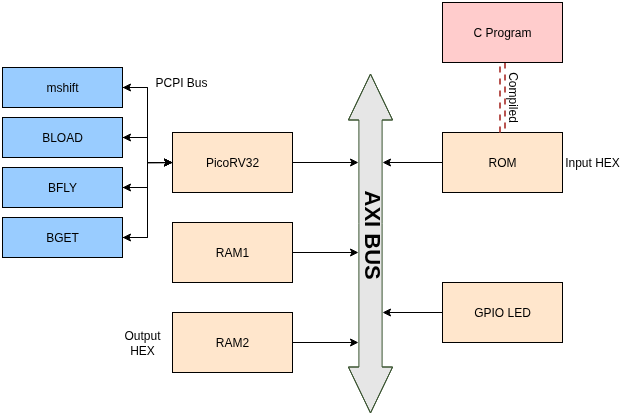
\includegraphics[width=0.9\columnwidth]{Hardware architecture rtl.png}
\caption{Block diagram of the PicoRV32-based audio equalizer SoC with PCPI FFT custom instruction module.}
\label{fig:soc}
\end{figure}
The complete SoC is implemented in Verilog and simulated using Icarus Verilog.
The system architecture comprises:
\begin{itemize}
    \item PicoRV32 core: 32-bit RV32I implementation with PCPI enabled.
    \item PCPI FFT module: implements \texttt{bload}, \texttt{bfly}, \texttt{bget} as described in Section IV.
    \item ROM: 32 KB instruction memory loaded with the compiled audio equalizer program.
    \item Input RAM: stores the 1024-sample test audio waveform.
    \item Output RAM: 4 KB block for capturing the processed audio output stream (accessed via \texttt{MAGIC\_ADDR 0x00020000}).
    \item AXI bus: provides addressable interconnection between the core, memories, and GPIO peripherals.
\end{itemize}

% =============================================================
% SECTION 3.4 (Hardware Implementation) — bfly Verilog excerpt Extracted from
% picorv32_pcpi_fft.v. Requires \usepackage{listings} and the
% \lstdefinestyle{verilog}{...} block in the preamble.
% =============================================================

% --- Introducing paragraph (place before the listing) ---

Among the four custom instructions, \texttt{bfly} carries the arithmetic core of
the butterfly and is therefore the most representative of the hardware design.
The PCPI module decodes it when the instruction word carries opcode
\texttt{0x2B} and \texttt{funct3}~=~\texttt{1}, interpreting \texttt{rs1} as the
cosine twiddle term $c$ and \texttt{rs2} as the sine term $s$. These are
combined with the real and imaginary operands \texttt{s\_real\_64} and
\texttt{s\_imag\_64} that were captured by a preceding \texttt{bload}.
Listing~\ref{lst:bfly} shows the relevant portion of the Verilog implementation.

\begin{lstlisting}[style=PictureStyle,caption={Verilog implementation of the \texttt{bfly} custom instruction.},label={lst:bfly}]
wire signed [63:0] r_c = s_real_64 * c_64; 
wire signed [63:0] i_s = s_imag_64 * s_64; 
wire signed [63:0] r_s = s_real_64 * s_64; 
wire signed [63:0] i_c = s_imag_64 * c_64; 

wire signed [63:0] ti_64 = r_s + i_c;

wire signed [31:0] tr_result = tr_64[FIXED_SHIFT +: 32]; 
wire signed [31:0] ti_result = ti_64[FIXED_SHIFT +: 32];

else if (is_bfly) begin 
cached_ti  <= ti_result; 
pcpi_rd    <= tr_result; 
pcpi_wr    <= 1'b1; 
pcpi_ready <= 1'b1; 
end
\end{lstlisting}

A single \texttt{bfly} instruction serves both the forward and inverse transform
stages of the equalizer pipeline, with no dedicated inverse-FFT hardware. This
reuse follows directly from the relationship between the forward and inverse DFT
kernels. The forward transform applies the twiddle factor $W_{N}^{r} = e^{-j2\pi
r/N} = c - js$, whereas the inverse transform applies its complex conjugate
$W_{N}^{-r} = e^{+j2\pi r/N} = c + js$, where $c = \cos(2\pi r/N)$ and $s =
\sin(2\pi r/N)$. The cosine term $c$ is identical for both directions; only the
sign of the sine term $s$ differs.


The PCPI output signals \texttt{pcpi\_rd}, \texttt{pcpi\_wr}, and
\texttt{pcpi\_ready} are registered rather than driven combinationally. A
combinational \texttt{pcpi\_ready} can glitch when the decode signals settle
within a cycle, and because the PicoRV32 core samples \texttt{pcpi\_ready} at
the clock edge such a glitch could cause the instruction to be acknowledged
incorrectly. Registering the outputs guarantees a clean, stable handshake at
every clock edge, at the cost of one additional cycle of latency: an instruction
presented on \texttt{pcpi\_valid} in cycle $N$ produces its result and asserts
\texttt{pcpi\_ready} in cycle $N{+}1$.

\subsection{Software Integration}

To seamlessly bridge the high-level audio equalizer application with the
underlying custom DSP hardware, the proposed instructions are exposed to the C
programming environment via inline assembly macros. This methodology provides
explicit, cycle-accurate control over the coprocessor invocation without
requiring extensive modifications to the GCC compiler's backend instruction
scheduler.
\begin{lstlisting}[style=PictureStyle, caption={C macros for invoking the custom FFT instructions}, label={lst:macros}]
#define hw_bload(real_val, imag_val) \
  __asm__ volatile ("bload %0, %1" :: \
    "r"((int32_t)(real_val)), \
    "r"((int32_t)(imag_val)) : "memory")

#define hw_bfly(tr_out, c_val, s_val) \
  __asm__ volatile ("bfly %0, %1, %2" \
    : "=r"(tr_out) \
    : "r"((int32_t)(c_val)), \
      "r"((int32_t)(s_val)) : "memory")

#define hw_bget(ti_out) \
  __asm__ volatile ("bget %0" \
    : "=r"(ti_out) :: "memory")
\end{lstlisting}

To enable the assembler to recognize the new mnemonics, the
\texttt{opcodes/riscv-opc.c} source file in GNU binutils was modified to add
entries for \texttt{bload}, \texttt{bfly}, and \texttt{bget} with their
corresponding encoding fields. The modified binutils is rebuilt and used in
place of the standard toolchain when compiling FFT code.

\section{Results and Discussion}

\subsection{Compiler Synthesis and Instruction Validation}

To verify the successful integration of the custom toolchain and the high-level
C macros, the compiled binary was disassembled and analyzed using the RISC-V GNU
objdump utility. The primary objective of this verification was to ensure that
the GCC compiler respected the sequential integrity of the custom DSP operations
without injecting redundant memory spills or reordering the instructions.

As shown in Fig.~\ref{fig:objdump}, the disassembled object code confirms the
flawless translation of the C macros into the reserved \texttt{0x2B} custom
opcode space. Crucially, the compiler successfully fetches the array values into
registers \texttt{(a4, a5)} and immediately feeds them into the \texttt{bload}
instruction. Protected by the inline assembly memory barriers, the subsequent
\texttt{bfly} and \texttt{bget} instructions are emitted in perfect consecutive order.

\begin{figure}[!ht]
\centering
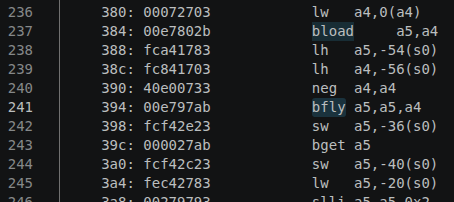
\includegraphics[width=0.9\columnwidth]{custom instructions.png}
\caption{Assembly output generated from the compiler showing the correct custom instructions \texttt{bload}, \texttt{bfly}, and \texttt{bget} with proper register usage.}
\label{fig:objdump}
\end{figure}

While necessary memory operations such as \texttt{sw} (store word) and \texttt{lw} (load word) are
natively present to update the final array values, the disassembled code
provides empirical proof that all redundant intermediate register spilling has
been successfully eliminated. The \texttt{bload}, \texttt{bfly}, and
\texttt{bget} sequence flawlessly executes the complex four-variable Butterfly
computation without ever requiring the CPU to temporarily offload incomplete
arithmetic states to the RAM. By effectively confining the intense mathematical
cross-multiplications entirely within the coprocessor's hardware state, the
system successfully bypasses the bottleneck and is fully optimized
for the cycle-accurate performance evaluation detailed in the subsequent
section.

\subsection{Functional Correctness Verification}

The hardware-accelerated FFT output was verified against a double-precision
floating-point reference implemented in Python using NumPy's \texttt{fft} and
\texttt{ifft} functions on identical input data. The Python reference applied
the same 3-band equalizer gain pattern ($2.0\times$, $0.5\times$, $0.25\times$
in Q10) to ensure direct comparison.

Each 32-bit Q21.10 fixed-point output sample from the hardware simulation was
converted to floating-point by dividing by $2^{10} = 1024$ prior to comparison.
Error metrics over the 1024-sample output sequence are presented in
Table~\ref{tab:correctness}.

\begin{table}[h!]
\caption{Correctness Verification Metrics}
\label{tab:correctness}
\centering
\begin{tabular}{@{}lr@{}}
\toprule
\textbf{Metric} & \textbf{Value} \\
\midrule
Samples compared                 & 1024 \\
Maximum absolute error           & 4.94 \\
Mean absolute error              & 0.92 \\
RMS error                        & 1.30 \\
Mean relative error              & 0.28\% \\
SNR (hardware vs.\ reference)    & 56.28 dB \\
\bottomrule
\end{tabular}
\end{table}

The error metrics in Table~\ref{tab:correctness} confirm that the fixed-point
hardware implementation produces results consistent with the double-precision
floating-point reference. The 56.28~dB signal-to-noise ratio indicates that the
signal energy exceeds the error energy by more than a factor of $4 \times
10^{5}$, and the mean relative error of 0.28\% shows that, on average, each
output sample deviates from the reference by well under one percent. This
residual error does not originate from any computational fault but from the
deliberate use of fixed-point arithmetic. The reference, by contrast, uses
64-bit double-precision arithmetic with effectively no rounding. A small,
bounded deviation between the two is therefore expected.

An SNR of 56.28~dB thus represents a high-fidelity match to the reference,
sufficient for the gain-adjustment task of an audio equalizer, so the error is
acceptable and the custom-instruction FFT can be considered functionally correct
relative to the floating-point reference.

\subsection{Performance Comparison}

The complete audio equalizer SoC was synthesized in two configurations to
quantify the hardware cost of the proposed extension. Both were synthesized for
the Xilinx Zynq-7020 device in Vivado 2025.1 under an identical 20 ns (50 MHz)
clock constraint, and the two builds are identical in every respect except for
the custom instruction module. The difference between the two configurations
therefore isolates the cost of the proposed instructions.
Table~\ref{tab:resource} reports the comparison across computational
performance, occupied slices, total on-chip power, and maximum operating
frequency.

\begin{table}[h!]
\centering
\caption{Resource and performance comparison}
\label{tab:resource}
\begin{tabular}{@{}lccc@{}}
\toprule
Metric & Baseline & With custom inst. & Change \\
\midrule
FFT computation (M cycles) & 17.08  & 5.84  & 65.8\% \\
Chip area (slices)         & 11678  & 11979 & 2.60\% \\
Total on-chip power (mW)   & 132    & 136   & 3.03\% \\
$f_{\max}$ (MHz)           & 56.9   & 55.8  & -1.93\% \\
\bottomrule
\end{tabular}
\end{table}

The results show that the 65.8\% or 2.92× acceleration of the FFT computation is
obtained at a small hardware cost. The number of occupied slices increases by
only 2.60\%, from 11,678 to 11,979. The hardware cost in power and frequency is
similarly limited. Total on-chip power rises by 3.03\%, from 132 mW to 136 mW.
This increase is attributable entirely to the additional dynamic switching
activity of the custom instruction module. The maximum operating frequency
decreases by 1.93\%, from 56.9 MHz to 55.8 MHz, reflecting the slightly longer
critical path of the wide butterfly multipliers. 

Both configurations nonetheless meet all timing constraints at the target
frequency. Taken together, these results indicate that the proposed custom
instructions reduce FFT computation time by 65.8\% while increasing area by only
2.60\% and total power by 3.03\%, demonstrating that profile-driven custom
instruction design delivers a favorable performance-to-cost trade-off on a
minimal RISC-V core.

\section{Conclusion}

This paper presented a profile-driven design and implementation of custom RISC-V
instructions for accelerating Fast Fourier Transform computation in an audio
equalizer application. Four custom instructions \texttt{mshift}, \texttt{bload},
\texttt{bfly}, and \texttt{bget} collapse the four-input, two-output butterfly
operation into a single hardware-accelerated sequence and minimize the
multiplication operations, integrated through the standard PCPI interface
without modifying the PicoRV32 core. Static instruction profiling identified the
butterfly multiplication as the dominant bottleneck, motivating the choice of
acceleration target. Experimental results from Icarus Verilog simulation show a
2.92$\times$ cycle count reduction for processing 1024 audio samples through a
64-point FFT-based equalizer, compared to the RV32I software-only baseline. The
GNU binutils assembler was modified to recognize the custom mnemonics, enabling
clean integration through inline assembly without compiler backend changes.

Future work will address three extensions. First, hardware acceleration of the
bit reversal stage to capture additional cycle savings. Second, FPGA synthesis
to characterize area and power overhead. Third, evaluation with larger FFT sizes
($N = 128, 256$) to assess scalability of the speedup.

\begin{thebibliography}{00}
\bibitem{stefani2022}
D. Stefani and L. Turchet, ``On the challenges of embedded real-time music information retrieval,'' in \emph{Proc. 25th Int. Conf. Digital Audio Effects (DAFx20in22)}, Vienna, Austria, 2022.
\bibitem{cooley1965}
J. W. Cooley and J. W. Tukey, ``An algorithm for the machine calculation of complex Fourier series,'' \emph{Math. Comput.}, vol. 19, no. 90, pp. 297--301, 1965.
\bibitem{oppenheim}
A. V. Oppenheim and R. W. Schafer, \emph{Discrete-Time Signal Processing}, 3rd ed. Upper Saddle River, NJ, USA: Pearson, 2010.
\bibitem{waterman2019}
A. Waterman, K. Asanovic, and J. Hauser, \emph{The RISC-V Instruction Set Manual: Volume I: Unprivileged ISA}, Document Version 20191213, RISC-V Foundation, 2019.
\bibitem{cao2025}
P. Cao, H. Wang, H. Cao, Z. Wu, and Y. Liu, ``A flexible dual-mode and efficient RISC-V coprocessor for on-node FFT acceleration in edge sensing,'' \emph{IEEE Embedded Syst. Lett.}, 2025, doi: 10.1109/LES.2025.3634524.
\bibitem{hu2021}
B. Hu, Y. Chen, and X. Zeng, ``An agile instruction set extension method based on the RISC-V processor,'' in \emph{Proc. 2021 IEEE 4th Int. Conf. on Electronics Technology (ICET)}, 2021, pp. 1--5, doi: 10.1109/ICET51757.2021.9450911.
\bibitem{yuan2022}
J. Yuan, Q. Zhao, W. Wang, X. Meng, J. Li, and Q. Li, ``Audio denoising coprocessor based on RISC-V custom instruction set extension,'' \emph{WSEAS Trans. Commun.}, vol. 21, pp. 189--195, Jun. 2022, doi: 10.37394/23204.2022.21.23.
\bibitem{belhadj2022}
H. Belhadj Amor, C. Bernier, and Z. P\v{r}ikryl, ``A RISC-V ISA extension for ultra-low power IoT wireless signal processing,'' \emph{IEEE Trans. Comput.}, vol. 71, no. 4, pp. 766--778, Apr. 2022, doi: 10.1109/TC.2021.3063027.
\bibitem{picorv32}
C. Wolf, ``PicoRV32---A size-optimized RISC-V CPU,'' GitHub repository. [Online]. Available: \url{https://github.com/YosysHQ/picorv32}
\bibitem{cui2023}
E. Cui, T. Li, and Q. Wei, ``RISC-V instruction set architecture extensions: A survey,'' \emph{IEEE Access}, vol. 11, pp. 24696--24711, Mar. 2023, doi: 10.1109/ACCESS.2023.3246491.
\bibitem{wang2024}
S. Wang, X. Wang, Z. Xu, B. Chen, C. Feng, Q. Wang, and T. T. Ye, ``Optimizing CNN computation using RISC-V custom instruction sets for edge platforms,'' \emph{IEEE Trans. Comput.}, vol. 73, no. 5, pp. 1371--1384, May 2024, doi: 10.1109/TC.2024.3362060.
\bibitem{garofalo2021}
A. Garofalo, G. Tagliavini, F. Conti, L. Benini, and D. Rossi, ``XpulpNN: Enabling energy efficient and flexible inference of quantized neural networks on RISC-V based IoT end nodes,'' \emph{IEEE Trans. Emerg. Topics Comput.}, vol. 9, no. 3, pp. 1489--1505, Jul.--Sep. 2021, doi: 10.1109/TETC.2021.3072337.
\bibitem{mousavikia2022}
S. K. Mousavikia, E. Gholizadehazari, M. Mousazadeh, and S. B. Ors Yalcin, ``Instruction set extension of a RiscV based SoC for driver drowsiness detection,'' \emph{IEEE Access}, vol. 10, pp. 58151--58162, May 2022, doi: 10.1109/ACCESS.2022.3177743.
\bibitem{chen2024}
Y. Chen, X. Wang, S. Song, L. Feng, and Z. Wang, ``RISC-V custom instructions of elementary functions for IoT endpoint devices,'' \emph{IEEE Trans. Comput.}, vol. 73, no. 2, pp. 523--535, Feb. 2024, doi: 10.1109/TC.2023.3336174.
\bibitem{cmlabfft}
Communication \& Multimedia LAB, NTU, ``Fast Fourier Transform (FFT).'' [Online]. Available: \url{https://www.cmlab.csie.ntu.edu.tw/cml/dsp/training/coding/transform/fft.html} [Accessed: May 16, 2026].
\bibitem{riscvprofiler}
V. Mahendra, ``riscv-application-profiler,'' GitHub repository, 2023. [Online]. Available: \url{https://github.com/mahendraVamshi/riscv-application-profiler} [Accessed: May 16, 2026].

\end{thebibliography}
\end{document}
